\chapter{Mapping Integer Linear Programs to Einsum}
\label{chap:appendix:map_ilp}

First translate the ILP
\begin{gather*}
    \min_{x \in \mathbb{Z}_+^n} c^\T x\\
    \text{s.t.} Ax = b
\end{gather*}
to a QUBO
$$\min_{\overline{x} \in \smallset{0,1}^m} \overline{x}^\T Q \overline{x}$$
by
\begin{enumerate}[label={\arabic*.}]
    \item binarizing the input $x \in \mathbb{Z}_+^n$ to $\overline{x} \in \smallset{0,1}^m$ with an upper bound on $x$,
    \item turning the constraints $$Ax = b$$ to penalties in the objective function $$\rho (Ax - b)^\T (Ax - b)$$ for a big enough $\rho \in \R$, and
    \item embedding linear terms on the diagonal of $Q$.
\end{enumerate}

Then consider a symbol $s_i \in S$ for each row $i \in [m]$ of $\overline{x}$.
We introduce a factor $T^{(k, k)}$ with index string $\bm{s_{kk}} = s_k$ for every diagonal entry, and a factor $T^{(i,j)}$ with index string $\bm{s_{ij}} = s_i s_j$ for every non-diagonal entry:
\begin{align*}
    T^{(k, k)} & := \begin{pmatrix}
        0 \\
        q_{kk}
    \end{pmatrix} \\
    T^{(i,j)}  & := \begin{pmatrix}
        0 & 0      \\
        0 & q_{ij}
    \end{pmatrix}
\end{align*}
We can then solve the QUBO by computing the Einsum expression
$$(\bm{s_{11}}, \dots, \bm{s_{1m}}, \dots, \bm{s_{m1}}, \dots, \bm{s_{mm}} \rightarrow, T^{(1,1)}, \dots, T^{(1,m)}, \dots, T^{(m,1)}, \dots, T^{(m, m)})$$
over the semiring $R = (\R, \min, +)$.

\begin{figure}[h]
    \centering
    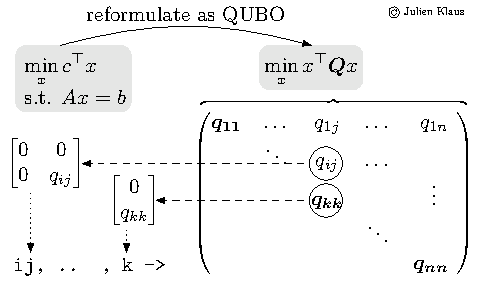
\includegraphics{graphics/ilp.pdf}
    \caption{Translation of ILP to Einsum \copyright Julien Klaus}
    \label{fig:appendix:map_ilp:ilp_to_einsum}
\end{figure}